% This is "sig-alternate.tex" V2.0 May 2012
% This file should be compiled with V2.5 of "sig-alternate.cls" May 2012
%
% This example file demonstrates the use of the 'sig-alternate.cls'
% V2.5 LaTeX2e document class file. It is for those submitting
% articles to ACM Conference Proceedings WHO DO NOT WISH TO
% STRICTLY ADHERE TO THE SIGS (PUBS-BOARD-ENDORSED) STYLE.
% The 'sig-alternate.cls' file will produce a similar-looking,
% albeit, 'tighter' paper resulting in, invariably, fewer pages.
%
% ----------------------------------------------------------------------------------------------------------------
% This .tex file (and associated .cls V2.5) produces:
%       1) The Permission Statement
%       2) The Conference (location) Info information
%       3) The Copyright Line with ACM data
%       4) NO page numbers
%
% as against the acm_proc_article-sp.cls file which
% DOES NOT produce 1) thru' 3) above.
%
% Using 'sig-alternate.cls' you have control, however, from within
% the source .tex file, over both the CopyrightYear
% (defaulted to 200X) and the ACM Copyright Data
% (defaulted to X-XXXXX-XX-X/XX/XX).
% e.g.
% \CopyrightYear{2007} will cause 2007 to appear in the copyright line.
% \crdata{0-12345-67-8/90/12} will cause 0-12345-67-8/90/12 to appear in the copyright line.
%
% ---------------------------------------------------------------------------------------------------------------
% This .tex source is an example which *does* use
% the .bib file (from which the .bbl file % is produced).
% REMEMBER HOWEVER: After having produced the .bbl file,
% and prior to final submission, you *NEED* to 'insert'
% your .bbl file into your source .tex file so as to provide
% ONE 'self-contained' source file.
%
% ================= IF YOU HAVE QUESTIONS =======================
% Questions regarding the SIGS styles, SIGS policies and
% procedures, Conferences etc. should be sent to
% Adrienne Griscti (griscti@acm.org)
%
% Technical questions _only_ to
% Gerald Murray (murray@hq.acm.org)
% ===============================================================
%
% For tracking purposes - this is V2.0 - May 2012

\documentclass{sig-alternate}

\usepackage{xcolor}
\newcommand\todo[1]{\textcolor{red}{#1}}


\begin{document}
%
% --- Author Metadata here ---
\conferenceinfo{SIGIR}{'14 Gold Coast, Australia}
%\CopyrightYear{2007} % Allows default copyright year (20XX) to be over-ridden - IF NEED BE.
%\crdata{0-12345-67-8/90/01}  % Allows default copyright data (0-89791-88-6/97/05) to be over-ridden - IF NEED BE.
% --- End of Author Metadata ---

\title{On a Tip of Your Search: Evaluating Effect of Search Tips for Complex Informational Search Tasks}

%
% You need the command \numberofauthors to handle the 'placement
% and alignment' of the authors beneath the title.
%
% For aesthetic reasons, we recommend 'three authors at a time'
% i.e. three 'name/affiliation blocks' be placed beneath the title.
%
% NOTE: You are NOT restricted in how many 'rows' of
% "name/affiliations" may appear. We just ask that you restrict
% the number of 'columns' to three.
%
% Because of the available 'opening page real-estate'
% we ask you to refrain from putting more than six authors
% (two rows with three columns) beneath the article title.
% More than six makes the first-page appear very cluttered indeed.
%
% Use the \alignauthor commands to handle the names
% and affiliations for an 'aesthetic maximum' of six authors.
% Add names, affiliations, addresses for
% the seventh etc. author(s) as the argument for the
% \additionalauthors command.
% These 'additional authors' will be output/set for you
% without further effort on your part as the last section in
% the body of your article BEFORE References or any Appendices.

\numberofauthors{2} 

\author{
% 1st. author
\alignauthor
Denis Savenkov\\
       \affaddr{Emory University}\\
       \email{dsavenk@emory.edu}
% 2nd. author
\alignauthor
Eugene Agichtein\\
       \affaddr{Emory University}\\
       \email{eugene@mathcs.emory.edu}
}
\date{17 February 2014}
% Just remember to make sure that the TOTAL number of authors
% is the number that will appear on the first page PLUS the
% number that will appear in the \additionalauthors section.

\maketitle
\begin{abstract}
Search engine is a ubiquitous tool used by millions of people on a daily basis.
However, as with every tool, certain skills are required in order to use it efficiently.
Unfortunately users have different experience and not everybody is able to find answers to all questions she is interested in \todo{[find a paper to cite here]}.
Helping users to develop their search skills was included as one of the key research directions by \cite{Allan:2012:FCO:2215676.2215678}. However, the assistance offered by the modern search engines are limited to query suggestion and spelling correction \todo{[something else?]}.
A number of researches are available that study different ways of helping users be more successful with their searches \todo{[cite some reviews, or a couple of different papers]}. 
In this work we study the effect of showing users search tips designed to help asking the better queries when solving a difficult informational search task.
We show that ``the right'' tips can improve users' success rate.
However generic hints might be misleading and detrimental to user search experience.
\end{abstract}

% A category with the (minimum) three required fields
\category{H.3.3}{Information storage and retrieval}{Information Search and Retrieval}[query formulation, search process]
%A category including the fourth, optional field follows...

\terms{Measurement, Design, Experimentation, Human Factors}

\keywords{User studies, search interface, experimental design, effectiveness measures, query reformulation, expertise, tactics, tips, suggestions, assistance, efficiency.}

\section{Introduction}
\todo{Motivation of search hints as alternative/addition to query suggestion, especially for tasks when search cannot be solved with a single query}

Improving user search experience is usually considered as a problem of improving retrieval performance. 

\todo{Query suggestion is similar to tips, but is not guaranteed to be good, usually rely on more behavior data available for the new query}

\todo{Query terms selection}

\todo{Other dialog systems?}

\todo{Showing predicted retrieval performance}

\todo{Search snippets}


\section{Related Work}
\todo{Based on related work review from Daniel Russel \cite{Moraveji:2011:MIU:2009916.2009966}}.

\todo{Summarize works on task level query suggestion}
Experiment Design
\todo{State main difference from Dan Russel paper: we focus on informational tasks which are solved with web search and hints are less likely to be 100\% helpful}

\section{Tips for Difficult Search Tasks}
To estimate the effect of search tips on user behavior and success we conducted a user study using Amazon Mechanical Turk platform\footnote{http://www.mturk.com/}. 
The motivation to find the correct answer is very important for the study, thus we decided to pose it as a web search game, similar to ``a Google a Day''\footnote{http://www.agoogleaday.com/} and uFindIt \cite{Ageev:2011:FYG:2009916.2009965}. 

\subsection{Web Search Game}
The web search game used for the study offers users to find answers to several questions using the provided web search interface. Figure \ref{figure:ufindit} shows the interface of the game.
% Rules
At the beginning of the game users were instructed to use only the search interface provided.
Answers should actually be found when using web search.
In a rare occurrence that user might know the answer to a question she is instructed to ignore the prior knowledge and find the answer anyway.
Since tasks might be difficult a chance to skip a question was provided, although users were instructed that effort put into solving a question will be evaluated.

In the previous experiments we've noticed that with difficult search tasks Mechanical Turk workers tend to skip the answer validation phase and submit the first hypothesis they found, although even shallow analysis reveals that it is incorrect.
To motivate deeper analysis of the candidates the final version of the game featured automatic answer verification. Each answer submitted by a user was checked for the presence of the required keyword.
If the answer was incorrect a dialog popped up and a player could continue search.

% Technology
The game search interface was based on API of one of the major web search engines. All search results were cached so that users asking the same query get the same results. Moreover, all links to web pages were rewritten to use our caching HTTP proxy.

% Finally
At the end of the game a questionnaire was presented asking for feedback on user satisfaction with the game, prior experience and other comments.

\begin{figure}
\centering
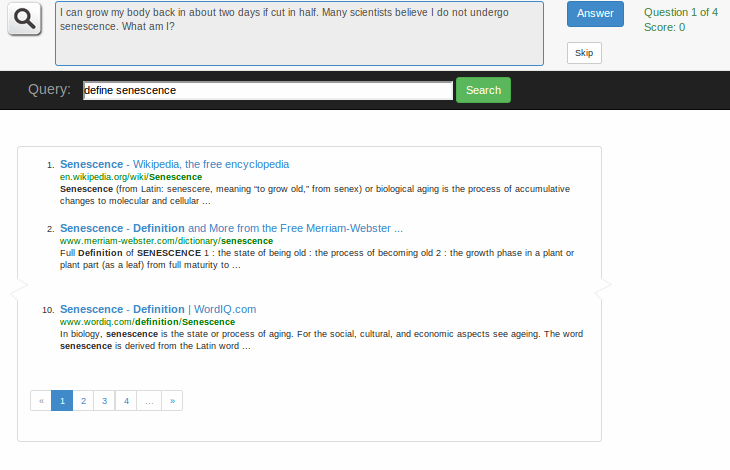
\includegraphics[scale=0.29]{img/ufindit}
\caption{The interface of the UFindIt game}
\label{figure:ufindit}
\end{figure}

\subsection{Search Tasks Description}

The tasks for the study were borrowed from the a Google a Day questions archive. Unfortunately, a lot of web pages exists that discuss solutions to these questions. Thus we had to filter search results excluding all pages that mentions the major part of the search questions or phrase ``a google a day''.
To keep users focused throughout the whole game we decided to limit the number of questions to 4.
Table \ref{table:tasks} describes all 4 tasks with the possible solutions. These tasks are quite difficult and usually involved more than one query to solve them with the game search interface.

\begin{table*}
\centering
\caption{Search tasks used for the study}
\label{table:tasks}
\begin{tabular}{|l|p{6cm}|p{8cm}|} \hline
Task ID & Task Text & Possible \\ \hline
Task 1 (``hydra'') & I can grow my body back in about two days if cut in half. Many scientists believe I do not undergo senescence. What am I? & Search [regenerative animal]. This will yield a number of possibilities including starfish, salamanders and several others. Search [senescence]. Find out that it means ``biological aging''. Search [animal biologically immortal], and learn that the hydra supposedly fulfill both of the above criteria. \\ \hline
Task 2 (``quirinus'') & Of the Romans "group of three" gods in the Archaic Triad, which one did not have a Greek counterpart? & Search for [Archaic Triad] to find Jupiter, Mars and Quirinus. Among those Quirinus didn't have a Greek counterpart.\\ \hline
Task 3 (``dinosaur'') & As George surveyed the ``waterless place'', he unearthed some very important eggs of what animal? & Search for [waterless place] to find out that it is the translation of the Mongolian word "Gobi" or ``Gobi Desert''. George Olsen unearthing the first whole dinosaur eggs in 1923. \\ \hline
Task 4 (``cherokee'') & If you were in the basin of the Somme River at summers end in 1918, what language would you have had to speak to understand coded British communications? & Search [somme river basin 1918]. Find out that's when the Second Battle of the Somme (a WWI battle) took place. Searching [second battle of somme code language] reveals the Cherokee served as code talkers in battle. They relayed messages in the Cherokee language that Germans couldn't decipher. \\ \hline
\end{tabular}
\end{table*}

\subsection{Search Tips}
The tasks used for the game are examples of complex informational search problems and usually require several searches. Questions have multiple parts and to solve them it is helpful to search for answers to parts of the questions and then combine them.

We studies 2 types of search tips: task specific and generic. Task specific hints were constructed from one of the possible solutions to the question and described one way to search and find the answer. Generic hint described the general strategy that can be applied to many difficult informational search task.
The actual tips shown to the players are described below.

Generic hint was the same for all tasks and looked the following way:
\begin{enumerate}
\item Split question into 2 or more logical parts
\item Find answers to the parts of the question
\item Use answers to the parts of the question to find answer to the full question
\end{enumerate}
For example:\\
Question: The second wife of King Henry VIII is said to haunt the grounds where she was executed. What does she supposedly have tucked under her arm?
\begin{enumerate}
\item Search [second wife King Henry VIII] to find Anne Boleyn.
\item Search [Anne Boleyn under arm] to find that her ghost is in the London Tower where she is said to carry her head tucked underneath her arm.
\end{enumerate}

Specific hints were designed for each question separately and presented a way to solve the problem by searching for a specific parts of the question.
Specific tip for Task 1:
\begin{enumerate}
\item Find what is senescence
\item Find who do not undergo senescence
\item Find animals who can regenerate body and choose the one that satisfy both conditions
\end{enumerate}

Tip for Task 2:
\begin{enumerate}
\item Find the names of the gods from the Archaic triad
\item For each of the gods find a Greek counterpart
\end{enumerate}

Tip for Task 3:
\begin{enumerate}
\item Find what is the ``waterless place'' mentioned in the question?
\item Search for important eggs discovery in this ``waterless place''
\end{enumerate}

To estimate the effect of search tips on users behavior and success we split users into 3 groups: users who were shown no hints; users who were shown task specific hints and users who were shown generic hint for all tasks.
To avoid the learning effect demonstrated in \cite{Moraveji:2011:MIU:2009916.2009966} we assign a user to a single group only.

\section{Results}
\todo{Provide raw results of the experiments, e.g. how many participants, how many HITs accepted, rejected, problems. Show examples of search trails for successful and unsuccessful searches}.

From 199 participants, who accepted the HIT on Amazon Mechanical Turk\footnote{http://mturk.com/}, only 169 moved further than the rules of the game and got to the first questions.
The search tasks were difficult and some players decided to quit the game, thus only 90 players finished the game, from those there were 9 submissions which we filtered out from the future analysis.
The only 2 reasons for that were: lack of effort, e.g. some players skipped several tasks after only a single query; some other submissions indicated usage of external resources such as outside of the game search engine, e.g. the only query asked was the correct answer to the task.
From 81 submissions 10 players indicated in the survey that they didn't see the tips which were shown to them, so we further filtered those submissions and finally we had 71 completed games, which split into the groups of 29, 20, 22 for players who didn't have tips, who had task-specific hints and who had generic tips correspondingly.


\subsection{Analysis}
\todo{Give a table and a couple of pictures with main quantitative results}

Figure \ref{figure:task_success} shows plots of the correct answers rate per task for groups of users who saw no hint, specific task-oriented hint or generic hint. As we can see, success rate is higher for users who saw specific hint than no hint at all. Somewhat surprising is the fact, that users who saw generic search hint were slightly less successful. The difference is more significant in more difficult tasks 1 and 4.

\begin{figure}
\centering
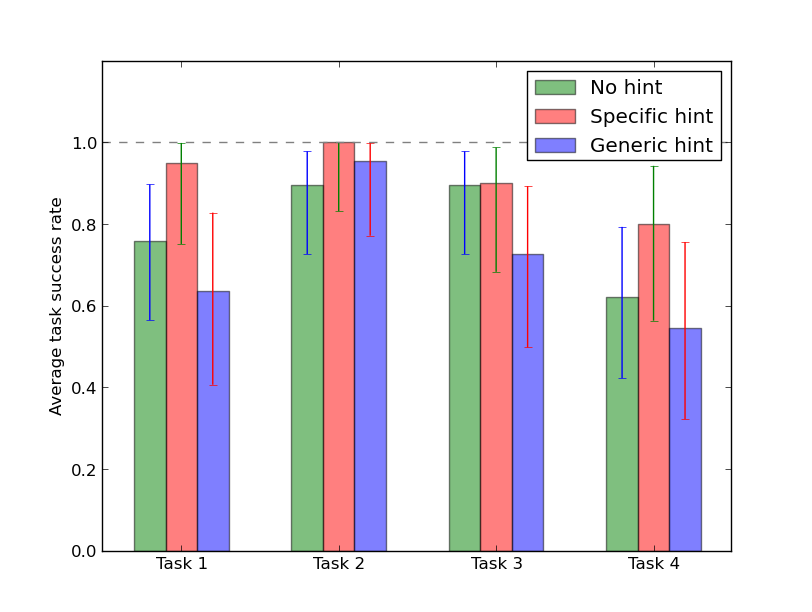
\includegraphics[scale=0.45]{img/success_per_task}
\caption{Success rate per task for each group of participants}
\label{figure:task_success}
\end{figure}

\begin{figure}
\centering
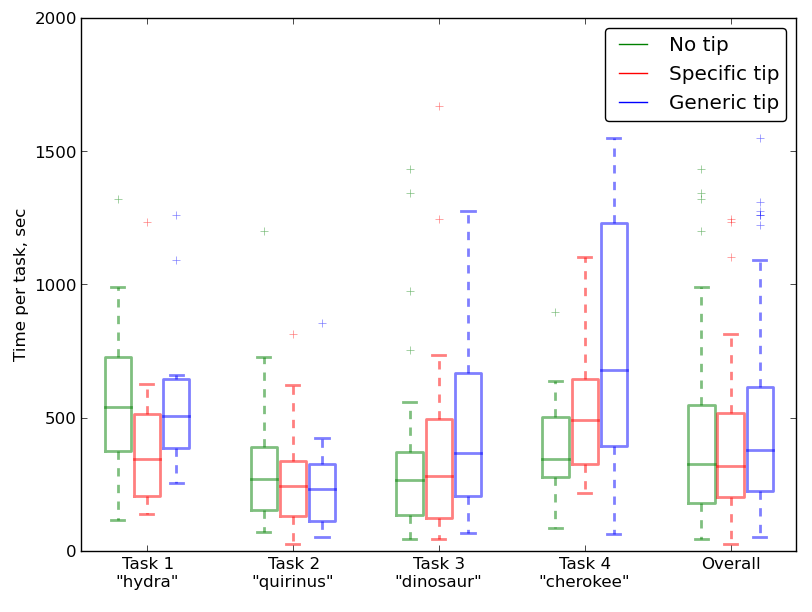
\includegraphics[scale=0.45]{img/time_per_task}
\caption{Task completion time for each group of players}
\label{figure:task_time}
\end{figure}


The main findings can be summarized as follows:
\begin{itemize}
\item ``Correct'' search tips allows users to find correct answer more often and do this faster than without search tips
\item ``General'' search hints can have detrimental effect on search success, reducing the success rate and increasing the time spent on task
\end{itemize}

\section{Discussions and Future Work}
\todo{Make a conclusion by summarizing the findings one more time}

\todo{Speculate on the negative effect of general search hints - distracting? hard to follow?, less satisfaction when tips were shown - self satisfaction?}. 

%ACKNOWLEDGMENTS are optional
\section{Acknowledgments}
Thanks to Dan Russel for sharing questions.

%
% The following two commands are all you need in the
% initial runs of your .tex file to
% produce the bibliography for the citations in your paper.
\bibliographystyle{abbrv}
\bibliography{sigproc}  % sigproc.bib is the name of the Bibliography in this case
% You must have a proper ".bib" file
%  and remember to run:
% latex bibtex latex latex
% to resolve all references
%
% ACM needs 'a single self-contained file'!
%
%APPENDICES are optional
%\balancecolumns

\end{document}
